% \special{dvipdfmx:config z 0}
\documentclass[UTF8,a4paper,AutoFakeBold,AutoFakeSlant]{article}
\usepackage[a4paper,left=2.8cm,right=2.6cm,top=3.7cm,bottom=3.5cm]{geometry}
\usepackage{ctex}
% \usepackage{xeCJK}
\usepackage{graphicx}
\usepackage{pythonhighlight}
\usepackage[mathscr]{eucal}
\usepackage{mathrsfs}
\usepackage{booktabs}
\usepackage{capt-of} 
\usepackage{hyperref} 
\usepackage{abstract}
\usepackage{amsmath}
\usepackage{listings}
\usepackage{color}
\usepackage{caption}
\usepackage{subfigure}
\usepackage{enumerate}
\usepackage{amsfonts} 
\usepackage{CJK,CJKnumb}
\usepackage{float}
% \usepackage{gbt7714}
\usepackage{framed}
\usepackage{multirow}
\usepackage{animate}
\usepackage[framemethod=tikz]{mdframed}



\newcommand{\song}{\CJKfamily{song}}    % 宋体   (Windows自带simsun.ttf)
\newcommand{\fs}{\CJKfamily{fs}}        % 仿宋体 (Windows自带simfs.ttf)
\newcommand{\kai}{\CJKfamily{kai}}      % 楷体   (Windows自带simkai.ttf)
\newcommand{\hei}{\CJKfamily{hei}}      % 黑体   (Windows自带simhei.ttf)
\newcommand{\li}{\CJKfamily{li}}        % 隶书   (Windows自带simli.ttf) 
\newcommand{\ssong}{\CJKfamily{STSong}}

\xeCJKsetup{SlantFactor = 0.3}
% \xeCJKsetup{SlantFactor = -0.7}
\setCJKmainfont[BoldFont=SimHei, SlantedFont=KaiTi]{SimSun}



% -- 中文字体 --
%\setCJKmainfont{Microsoft YaHei}  % 微软雅黑
%\setCJKmainfont{YouYuan}  % 幼圆
%\setCJKmainfont{NSimSun}  % 新宋体
%\setCJKmainfont{KaiTi}    % 楷体
% \setCJKmainfont{SimSun}   % 宋体
%\setCJKmainfont{SimHei}   % 黑体
% \setCJKfamilyfont{hwsong}{STSong}
 
% -- 英文字体 --
% \setmainfont{Times New Roman}
% \setmainfont{DejaVu Sans}
% \setmainfont{Latin Modern Mono}
% \setmainfont{Consolas}
% \setmainfont{Courier New}


\usepackage{xcolor}  	%高亮使用的颜色
\definecolor{commentcolor}{RGB}{85,139,78}
\definecolor{stringcolor}{RGB}{206,145,108}
\definecolor{keywordcolor}{RGB}{34,34,250}
\definecolor{backcolor}{RGB}{220,220,220}

\usepackage{accsupp}	
\newcommand{\emptyaccsupp}[1]{\BeginAccSupp{ActualText={}}#1\EndAccSupp{}}

\usepackage{listings}
\lstset{						%高亮代码设置
	language=python, 					%Python语法高亮
	linewidth=0.95\linewidth,      		%列表list宽度
	%basicstyle=\ttfamily,				%tt无法显示空格
	commentstyle=\color{commentcolor},	%注释颜色
	keywordstyle=\color{keywordcolor},	%关键词颜色
	stringstyle=\color{stringcolor},	%字符串颜色
	%showspaces=true,					%显示空格
	numbers=left,						%行数显示在左侧
	numberstyle=\tiny\emptyaccsupp,		%行数数字格式
	numbersep=5pt,						%数字间隔
	frame=single,						%加框
	framerule=0.1pt,						%划线
	escapeinside=@@,					%逃逸标志
	emptylines=1,						%
	xleftmargin=3em,					%list左边距
	backgroundcolor=\color{backcolor},	%列表背景色
	tabsize=4,							%制表符长度为4个字符
	% gobble=4							%忽略每行代码前4个字符
}




\renewcommand{\abstractname}{}    % clear the title
\renewcommand{\absnamepos}{empty}
%去除摘要两边缩进
\makeatletter
  \renewenvironment{abstract}{%
      \if@twocolumn
        \subsection*{\abstractname}%
      \else
        \small
        \begin{center}%
          {\bfseries \abstractname\vspace{-.5em}\vspace{\z@}}%
        \end{center}%
      \fi}
      {}
  \makeatother
\lstset{
  language=Matlab,
  keywords={break,case,catch,continue,else,elseif,end,for,function,
      global,if,otherwise,persistent,return,switch,try,while},
  basicstyle=\ttfamily,
  keywordstyle=\color{blue}\bfseries,
  commentstyle=\color{dkgreen},
  stringstyle=\color{dkpurple},
  backgroundcolor=\color{white},
  tabsize=4,
  showspaces=false,
  showstringspaces=false
}

\title{\textbf{\textsf{{\textsf{LB4} \heiti{机器学习概论}}}}} 
\author{\ssong PB19151769~~~~马宇骁}
\date{}

% 去掉红框
\hypersetup{
colorlinks=true,
linkcolor=black
}

\begin{document}



\maketitle

\tableofcontents
\newpage


% ----------------------------------section----------------------------------------------


\section{实验要求}

本次聚类实验主要实现的是《Clustering by fast search and find of density peaks》一文中的算法(以下简称DPC)

\begin{itemize}
  \item By Alex Rodriguez and Alessandro Laio
  \item Published on SCIENCE, 2014
  \item \url{https://sites.psu.edu/mcnl/files/2017/03/9-2dhti48.pdf}
\end{itemize}

本次实验的总体流程是完成 DPC 算法的代码实现,并在给定数据集上进行可视化实验。
\begin{enumerate}
  \item 读取数据集,(如有必要)对数据进行预处理
  \item 实现 DPC 算法,计算数据点的 $\delta_i$ 和 $\rho_i$
  \item 画出决策图,选择样本中心和异常点
  \item 确定分簇结果,计算评价指标,画出可视化图
\end{enumerate}

本次实验采用 Davis-Bouldin Index (DBI)(sklearn.metrics. davies\_bouldin\_score) 作为评价指标.






% ----------------------------------section----------------------------------------------

\section{实验原理}


\subsection{DPC算法}

DPC算法的两个假设为:
\begin{enumerate}
  \item 类簇中心被类簇中其他密度较低的数据点包围;
  \item 类簇中心间的距离相对较远。
\end{enumerate}


\subsubsection{局部密度}

假设N为样本个数,M为样本维数。
对于样本点i的局部密度,局部密度有两种计算方式,离散值采用截断核的计算方式,连续值则用高斯核的计算方式。

\begin{itemize}
  \item 截断核:
\end{itemize}

\begin{equation*}
  \rho_{i}=\sum_{i \neq j} \chi\left(d_{i j}-d_{c}\right)
\end{equation*}

\begin{equation*}
  \chi(x)=\left\{\begin{array}{ll}
    1, & x<0 \\
    0, & x \geq 0
    \end{array}\right.
\end{equation*}

\begin{itemize}
  \item 高斯核:
\end{itemize}

\begin{equation*}
  \rho_{i}=\sum_{i \neq j} \exp \left[-\left(\frac{d_{i j}}{d_{c}}\right)^{2}\right]
\end{equation*}

式中,di为数据点 i 与数据点 j 的欧氏距离,dc 为数据点 i 的邻域截断距离。
采用截断核计算的局部密度 $\rho_i$ 等于分布在样本点 i 的邻域截断距离范围内的样本点个数;
而利用高斯计算的局部密度 $\rho_i$ 等于所有样本点到样本点i的高斯距离之和。
DPC算法的原论文指出,对于较大规模的数据集,截断核的计算方式聚类效果较好;
而对于小规模数据集,高斯核的计算方式聚类效果更为明显。


\subsubsection{相对距离}

相对距离 $\delta_i$ 指样本点 i 与其他密度更高的点之间的最小距离。
在计算样本点 i 前需要对每个数据点的局部密度进行排序。

对于密度最高的样本,相对距离定义为:
$$ \delta_{i}=\max _{\mathrm{i} \neq \mathrm{j}}\left(\mathrm{d}_{\mathrm{ij}}\right) $$

对于其余数据点,相对距离定义为:
$$ \delta_{\mathrm{i}}=\min _{\mathrm{j}: \rho_{\mathrm{j}}>\rho_{\mathrm{i}}}\left(\mathrm{d}_{\mathrm{ij}}\right) $$

由于密度最高的样本不存在比其密度更高的点,DPC认为该点必为密度峰值(类簇中心),
人为设定其相对距离为最大值。剩余的密度峰值需要同时满足两个条件:局部密度 $\rho$ 较高,
相对距离 $\delta$ 较大。为此,DPC算法的原论文通过决策值 $\gamma$ 寻找这类密度峰值,下式给出
了 $\gamma_i$ 的定义:
$$ \gamma_i = \rho_i \times \delta_i $$

找到密度峰值后,DPC将剩余数据点分配给密度比它高的最近数据点所在类簇,形成多个从密度峰值出发的树状结构,每一个树状结构代表一个类簇。


\subsubsection{DPC算法的执行步骤}

\begin{enumerate}
  \item 利用样本集数据计算距离矩阵 dij;
  \item 确定邻域截断距离 dc;
  \item 计算局部密度 $\rho_i$ 和相对距离 $\delta_i$;
  \item 绘制决策图,选取聚类中心点;
  \item 对非聚类中心数据点进行归类,聚类结束。
\end{enumerate}

\subsection{DB指数 (Davies-Bouldin Index)}

如果真实标签未知,可以使用Davies-Bouldin Index(sklearn.metrics.davies\_bouldin\_score)来评估模型,其中较低的Davies-Bouldin值与具有更好的集群分离的模型。
这个指数表示集群之间的平均“相似度”,相似度是比较集群之间的距离和集群本身的大小的度量。
零分是最低分。接近于零的值表示更好的分区。

% Table generated by Excel2LaTeX from sheet 'Sheet1'
\begin{table}[htbp]
  \centering
    \begin{tabular}{|l|p{15.61em}|l|}
    \toprule
    参数    & \multicolumn{2}{c|}{说明} \\
    \midrule
    x     & \multicolumn{2}{p{25.22em}|}{array-like, shape (n\_samples,n\_features)\newline{}n\_features维数据点列表。每行对应一个数据点。} \\
    \midrule
    labels & \multicolumn{2}{p{25.22em}|}{array-like, shape (n\_samples,)\newline{}每个样本的预测标签。} \\
    \bottomrule
    \end{tabular}%
  \caption{sklearn.metrics.davies\_bouldin\_score}
  \label{tab:addlabel}%
\end{table}%

\begin{itemize}
  \item 返回值
\end{itemize}

float
所得的Davies-Bouldin得分。






% ----------------------------------section----------------------------------------------


\section{实验实现}


\subsection{实验调试}

针对三个数据集,由于算法思路相同,第一个数据集运行时间相对较久,所以没有采用再次确定聚类的簇数进行重新拟合。
对第二个和第三个进行了调试改进。

\begin{python}
  label1 = model1.fit()

  # label2 = model2.fit(method=None) # 四个聚类
  # label2 = model2.fit() # 10个聚类,还行
  label2 = model2.fit(findtype = 2, K=14) # 根据图像手动指定了14个

  # label3 = model3.fit() # 高斯4个聚类
  # label3 = model3.fit(method=None) # 5个聚类
  label3 = model3.fit(findtype = 2, K=7) # 根据图像手动指定了7个
\end{python}

其中,在定义的class DPC() 中拟合的时候当不指定局部密度计算的时候默认用高斯核。
\begin{python}
  # DPC算法拟合
  def fit(self, method="Gaussion", findtype = 1, K=1): # 指定1为find_centers_auto,2为find_centers_K(需要自己输入K)
      
      # 距离矩阵
      dists = self.getDistanceMatrix()
      dc = self.select_dc()
      # 计算局部密度
      rho = self.get_density(method = method)
      # 计算密度距离
      deltas, nearest_neiber = self.get_deltas()
      # 获取聚类中心点
      if findtype == 1:
          centers = self.find_centers_auto()
      elif findtype == 2:
          centers = self.find_centers_K(K = K)
      labs = self.cluster_PD()
      
      return labs
\end{python}



\subsection{实验结果}

最终,三个聚类的结果如下:

\begin{figure}[H]
	\centering
	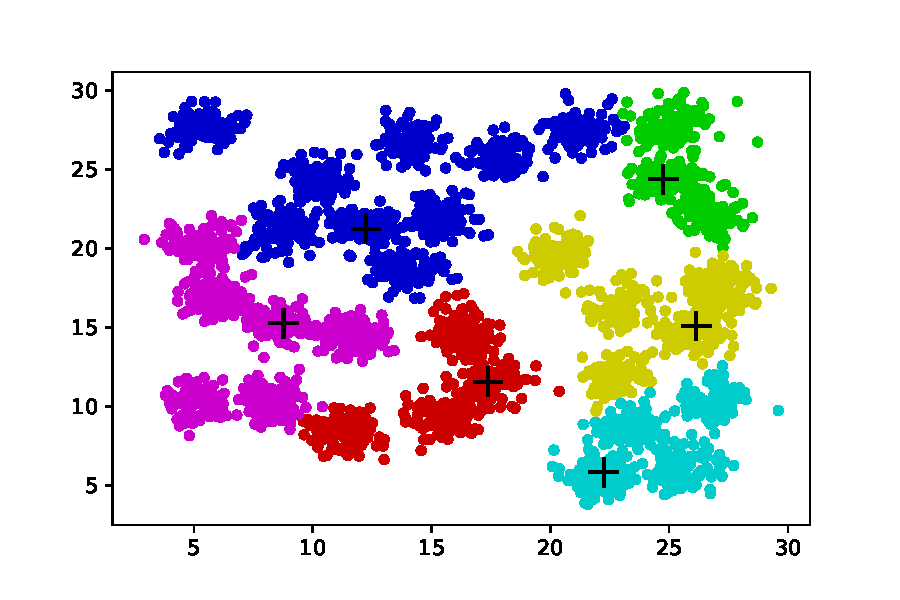
\includegraphics[scale=0.625]{cluster1.pdf}
	\caption{D31}
	\label{f:D31}
\end{figure}

\begin{figure}[H]
	\centering
	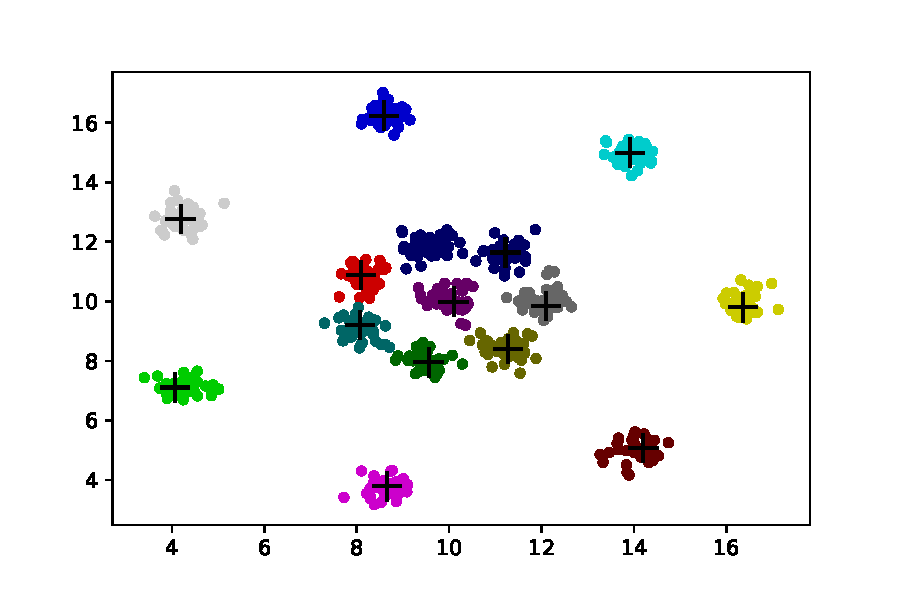
\includegraphics[scale=0.625]{cluster2.pdf}
	\caption{R15}
	\label{f:R15}
\end{figure}

\begin{figure}[H]
	\centering
	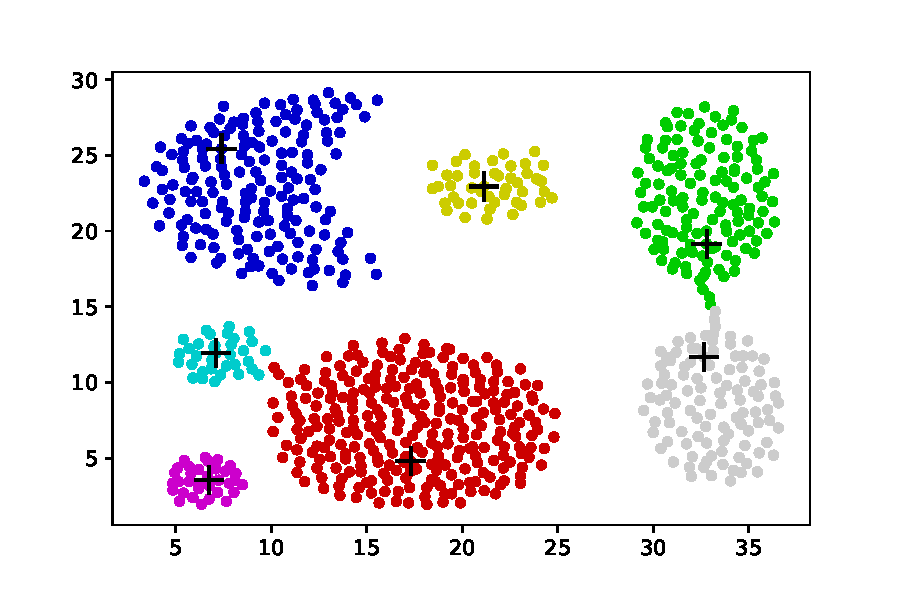
\includegraphics[scale=0.625]{cluster3.pdf}
	\caption{Aggregation}
	\label{f:Aggregation}
\end{figure}

\definecolor{shadecolor}{rgb}{0.92,0.92,0.92}
\begin{mdframed}[hidealllines=true,backgroundcolor=shadecolor]
\begin{verbatim}
  DBI(data1,label1), DBI(data2,label2), DBI(data3,label3)
  (0.781987832988031, 0.37374794009855516, 0.5035680502991704)
\end{verbatim}
\end{mdframed}

可以看到,后面两个聚类结果非常漂亮!




















% \bibliographystyle{gbt7714-numerical}
% % \bibliographystyle{7714-author-year}
% \bibliographystyle{ieeetr}
% \bibliography{bibl}

\end{document}